
\documentclass[a4paper,11pt]{article}

\usepackage{amsmath,amssymb,amsfonts,amsthm}    % Typical maths resource packages
\usepackage{graphicx}                           % Packages to allow inclusion of graphics
\usepackage{hyperref}                           % For creating hyperlinks in cross references
\usepackage[authoryear]{natbib}                 % literature reference style
\usepackage[bf]{caption2}




% -------------------------------
% --- some layout definitions ---
% -------------------------------

% define topline
\usepackage[automark]{scrpage2}
\pagestyle{scrheadings}
\automark{section}
\clearscrheadings
\ohead{\headmark}

% define citation style
\bibliographystyle{ecta}

% define page size, margin size
\setlength{\headheight}{1.1\baselineskip}
\voffset=-2cm
\hoffset=-3cm
\textheight24cm
\textwidth15.5cm
\topmargin1cm
\oddsidemargin3cm
\evensidemargin3cm

% define line line spacing = 1.5
\renewcommand{\baselinestretch}{1.5}

% define second level for `itemizing'
\renewcommand{\labelitemii}{-}




% --------------------------------------
% --------------------------------------
% --------------------------------------
% --- the structure the tex document ---
% ---  (this our recommendation) -------
% frontmatter:
%   - titlepage (mandatory),
%   - acknowledgement,
%   - abstract,
%   - table of contents (mandatory),
%   - list of abbreviations (not mandatory),
%   - list of figures (not mandatory),
%   - list of tables  (not mandatory) .
%
% body of the thesis (the structure of the thesis body is not mandatory, but the list of literature is mandatory):
%   - introduction,
%   - methods,
%   - data,
%   - results,
%   - conclusion,
%   - literature (mandatory),
%   - appendix (figures, tables).
%
% last page:
%   - declaration of authorship (mandatory).
% --------------------------------------
% --------------------------------------
% --------------------------------------

\begin{document}

% -------------------------------
% --- frontmatter: Title page ---
% -------------------------------

\thispagestyle{empty}
\begin{center}

    {\Large{\bf Bachelor's/Master's Thesis Title}} \vspace{0.5cm}


    {\normalsize Bachelor's/Master's Thesis submitted\\\vspace{0.5cm}
    to}\\\vspace{0.5cm}
    {\normalsize{\bf Prof. Dr. Nikolaus Hautsch}} \\\vspace{0.5cm}
    {\normalsize Humboldt-Universit\"at zu Berlin \\
    School of Business and Economics \\
    Institute for Statistics and Econometrics \\
    Chair of Econometrics} \vspace{1cm}


    {\normalsize by \\\vspace{0.5cm}
    {\bf your name} \\
    (your matriculation number)} \vspace{1cm}


    {\normalsize in partial fulfillment of the requirements \\
    for the degree of \\
    {\bf Bachelor/Master of Science} \\
    Berlin, September 30, 2007}

\end{center}




% ------------------------------------
% --- frontmatter: Acknowledgement ---
% ------------------------------------
\newpage
\pagestyle{plain}
\pagenumbering{roman}   % define page number in roman style
\setcounter{page}{1}    % start page numbering
\section*{Acknowledgement}

I would like to thank




% -----------------------------
% --- frontmatter: Abstract ---
% -----------------------------
\newpage
\section*{Abstract}

This is the template for a thesis at the Chair of Econometrics of
Humboldt--Universit\"at zu Berlin. A popular approach to write a
thesis or a paper is the IMRAD method (Introduction, Methods,
Results and Discussion). This approach is not mandatory! You can
find more information about formal requirements in the booklet
`Hinweise zur Gestaltung der \"au\ss eren Form von Diplomarbeiten'
which is available in the office of studies.\\

The abstract should not be longer than a paragraph of around 10 to
15 lines (or about 150 words). The abstract should contain a
concise description of the econometric/economic problem you
analyse and of your results. This allows the busy reader to obtain
quickly a clear idea of the thesis content.




% -----------------------------
% --- frontmatter: Contents ---
% -----------------------------
\newpage
\tableofcontents
\clearpage


% ----------------------------------------------------
% --- frontmatter: List of Figures (not mandatory) ---
% ----------------------------------------------------
\newpage
\addcontentsline{toc}{section}{List of Abbreviations}
\ohead[]{LIST OF ABBREVIATIONS}
\section*{List of Abbreviations}

\begin{table}[htbp]
\begin{tabular}{p{1cm} p{6.5cm} | p{1cm} p{6.5cm}}
    NGS     &  Next Generation Sequencing   & LNS     &  Laboratoire National de Sante  \\
    SGMB     &  Service of Genetics and Molecular Biology          & TST15     &  Illumina TruSight Tumor 15
\end{tabular}
\end{table}




% ----------------------------------------------------
% --- frontmatter: List of Figures (not mandatory) ---
% ----------------------------------------------------
\newpage
\addcontentsline{toc}{section}{List of Figures}
\ohead[]{\rightmark}
\listoffigures



% ---------------------------------------------------
% --- frontmatter: List of Tables (not mandatory) ---
% ---------------------------------------------------
\newpage
\addcontentsline{toc}{section}{List of Tables}
\listoftables



% -------------------------------
% --- main body of the thesis ---
% -------------------------------
\newpage
\pagestyle{plain}
\setcounter{page}{1}    % start page numbering anew
\pagenumbering{arabic}  % page numbers in arabic style


\section{Introduction}

  Cancer represents a huge burden for health care systems worldwide and one of
  the leading death causes. In 2012, there were an estimated 14.1 million new
  cancer cases with estimated  8.2 million cancer deaths
  {\cite{cancer_stats_worldwide:2012}}. Lung cancer is the most common cancer,
  both in terms of new cases (1.8 million) and deaths (1.6 million). Breast
  cancer is the second most common cancer (1.7 million cases) but only ranks 5th
  as cause of death (522,000 deaths). Colorectal cancer (1.4 million cases;
  694,000 deaths), prostate cancer (1.1 million cases; 307,000 deaths), stomach
  cancer (951,000 cases; 723,000 deaths) and liver cancer (782,000 cases;
  723,000 deaths) are following.

  Scientific discoveries in the last decade have had an enormous impact on our
  understanding of the underlying causes of cancer. The development of omics
  techniques, in combination with enhanced computational power, has lead to an
  explosion of biological data. It has become clear that cancer is an incredibly
  complex malignancy. The research community is trying to interprete this vast
  amount of data with the goal to get a deeper understanding of cancer and to
  cure it eventually. In recent years, several drugs have been approved that
  target proteins needed for cancer development, proliferation or metastasis.
  Molecular testing is employed to check whether these targeted drugs would be
  of benefit. In that regard, Next-Generation Sequencing (NGS) is an interesting
  method to gain deep insights into the genetic information of a tumor and to
  guide personalized therapy.

  \subsection{Cancer Genetics}

    Cancerogenesis is considered to be caused by an imbalance between the
    occurrence of mutations and cell-cycle control mechanisms, thereby leading
    to cardinal features of cancer: genomic instability and modifications. These
    alterations are caused either by inherited mutations or are acquired during
    cancerogenesis. Critical alterations include single nucleotide variations
    (SNVs), insertions and deletions of one or multiple nucleotides (INDELS),
    copy number variations (CNVs) and rearrangements.

    Genomic Instability

    Genomic Modifications

    Driver mutations

  \subsection{Targeting the EGFR Pathway in Solid Tumors}

    EGFR Pathway

    Targeted Drugs

    Resistances

  \subsection{Targeted Sequencing}

    \subsubsection{Target Enrichment Methods}

    \subsubsection{Illumina Sequencing Chemistry}

  \subsection{NGS Data Analysis}

    \subsubsection{GATK Best Practices}

  \subsection{Practical Implications in the Laboratory}

  \subsection{Aims of the Thesis}

\section{Method/Model/Theory}\label{Sec:Method}

\begin{itemize}

    \item How was the data analyzed ?

    \item Present the underlying economic model/theory and
        give reasons why it is suitable to answer the given problem.

    \item Present econometric/statistical estimation method and
        give reasons why it is suitable to answer the given problem.

    \item Allows the reader to judge the validity of the study and
        its findings.

    \item Depending on the topic this section can also be split up
        into separate sections.

\end{itemize}

\newpage
\section{Data}\label{Sec:Data}

\begin{itemize}

    \item Describe the data and its quality.
    \item How was the data sample selected?
    \item Provide descriptive statistics such as:
        \begin{itemize}
            \item time period,
            \item number of observations, data frequency,
            \item mean, median,
            \item min, max, standard deviation,
            \item skewness, kurtosis, Jarque--Bera statistic,
            \item time series plots, histogram.
        \end{itemize}
    \item For example:
        \begin{table}[ht]

        \begin{center}
            {\footnotesize
            \begin{tabular}{l|cccccccccc}
                \hline \hline
                           & 3m    & 6m    & 1yr   & 2yr   & 3yr   & 5yr   & 7yr   & 10yr  & 12yr  & 15yr   \\
                \hline
                    Mean   & 3.138 & 3.191 & 3.307 & 3.544 & 3.756 & 4.093 & 4.354 & 4.621 & 4.741 & 4.878  \\
                    StD    & 0.915 & 0.919 & 0.935 & 0.910 & 0.876 & 0.825 & 0.803 & 0.776 & 0.768 & 0.762  \\
                \hline \hline
            \end{tabular}}
        \end{center}
        \caption{Some descriptive statistics of location and dispersion for
        2100 observed swap rates for the period from February 15, 1999
        to March 2, 2007. Swap rates measured as 3.12 (instead of 0.0312). See Table
        \ref{Tab:DescripStatsRawDataDetail} in the appendix for
        more details.}
        \label{Tab:DescripStatsRawData}
        \end{table}

    \item Allows the reader to judge whether the sample is biased or to evaluate possible impacts of outliers, for
    example.

\end{itemize}

\newpage
\section{Results}\label{Sec:Results}

\begin{itemize}

    \item Organize material and present results.

    \item Use tables, figures (but prefer visual presentation):
        \begin{itemize}
            \item Tables and figures should supplement (and not duplicate) the
                text.

            \item Tables and figures should be provided with
            legends.\\
                {\it Figure \ref{Fig:Resids} shows how to include and reference
                graphics. The graphic must be labelled before. Files must be in
                \texttt{.eps} format.}

                \begin{figure}[ht]
                \begin{center}
                    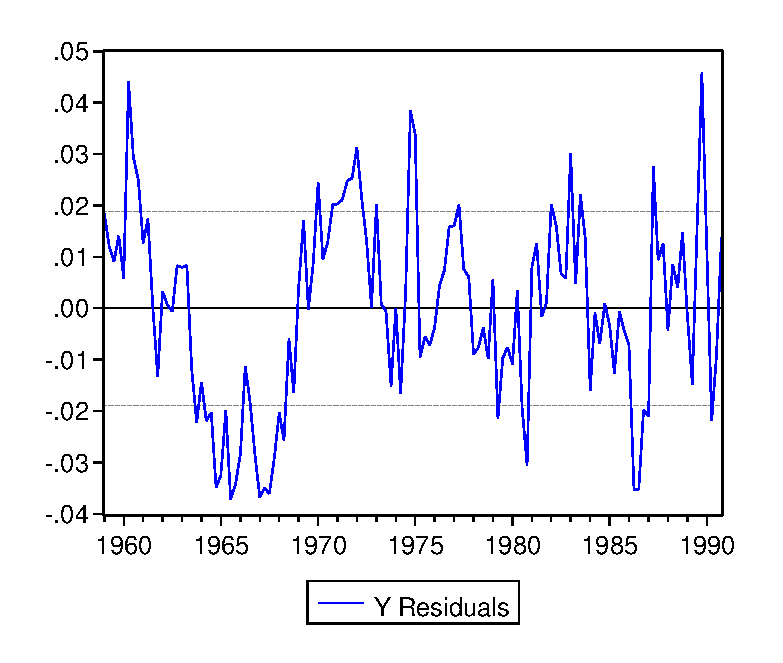
\includegraphics[scale=0.5,angle=0]{graph}
                    \caption{Estimated residuals from model XXX. ...}
                    \label{Fig:Resids}
                \end{center}
                \end{figure}

            \item Tables and graphics may appear in the text or in
                the appendix, especially if there are many simulation results
                tabulated, but is also depends on the study and number of tables resp.
                figures. The key graphs and tables must appear in
                the text!
        \end{itemize}

    \item Latex is really good at rendering formulas:\\
        {\it Equation (\ref{Eq:SpecDens}) represents the ACs of a stationary
        stochastic process:
        \begin{equation}
            f_y(\lambda) = (2\pi)^{-1} \sum_{j=-\infty}^{\infty}
                           \gamma_j e^{-i\lambda j}
                         =(2\pi)^{-1}\left(\gamma_0 + 2 \sum_{j=1}^{\infty}
        \gamma_j \cos(\lambda j)\right)
                                        \label{Eq:SpecDens}
        \end{equation}
        where $i=\sqrt{-1}$ is the imaginary unit, $\lambda \in [-\pi,
        \pi]$ is the frequency and the $\gamma_j$ are the autocovariances
        of $y_t$.}

\newpage

    \item Discuss results:
        \begin{itemize}
            \item Do the results support or do they contradict economic theory ?
            \item What does the reader learn from the results?
            \item Try to give an intuition for your results.
            \item Provide robustness checks.
            \item Compare to previous research.
        \end{itemize}
\end{itemize}

\section{Conclusions}\label{Sec:Conc}

\begin{itemize}

    \item Give a short summary of what has been done and what has been
    found.

    \item Expose results concisely.

    \item Draw conclusions about the problem studied. What are the
    implications of your findings?

    \item Point out some limitations of study (assist reader in judging validity
    of findings).

    \item Suggest issues for future research.

\end{itemize}




% ----------------
% --- appendix ---
% ----------------
\appendix

% literature
\newpage
\addcontentsline{toc}{section}{References}
\bibliography{literature}

% figures (not mandatory)
\newpage
\section{Figures}

\begin{figure}[ht]
    \begin{center}
        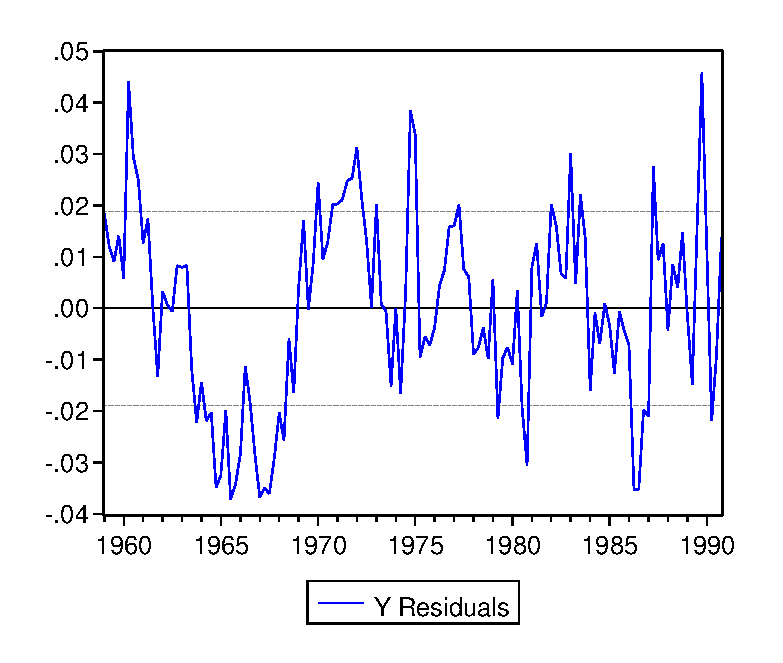
\includegraphics[scale=0.5,angle=0]{graph}
        \caption{Estimated residuals (2) from model XXX. ...}
        \label{Fig:Resids2}
    \end{center}
\end{figure}


% tables (not mandatory)
\newpage
\section{Tables}

\begin{table}[ht]
    \begin{center}
        {\footnotesize
        \begin{tabular}{l|cccccccccc}
        \hline \hline
                        & 3m    & 6m    & 1yr   & 2yr   & 3yr   & 5yr   & 7yr   & 10yr  & 12yr  & 15yr   \\
            \hline
                Mean   & 3.138 & 3.191 & 3.307 & 3.544 & 3.756 & 4.093 & 4.354 & 4.621 & 4.741 & 4.878  \\
                Median & 3.013 & 3.109 & 3.228 & 3.490 & 3.680 & 3.906 & 4.117 & 4.420 & 4.575 & 4.759  \\
                Min    & 1.984 & 1.950 & 1.956 & 2.010 & 2.240 & 2.615 & 2.850 & 3.120 & 3.250 & 3.395  \\
                Max    & 5.211 & 5.274 & 5.415 & 5.583 & 5.698 & 5.805 & 5.900 & 6.031 & 6.150 & 6.295  \\
                StD    & 0.915 & 0.919 & 0.935 & 0.910 & 0.876 & 0.825 & 0.803 & 0.776 & 0.768 & 0.762  \\
            \hline \hline
        \end{tabular}}
    \end{center}
    \caption{Detailed descriptive statistics of location and dispersion for
    2100 observed swap rates for the period from
    February 15, 1999 to March 2, 2007. Swap rates measured as 3.12 (instead of 0.0312).}
    \label{Tab:DescripStatsRawDataDetail}
\end{table}




% --------------------------------------------
% --- last page: Declaration of Authorship ---
% --------------------------------------------

\newpage
\thispagestyle{empty}
%{\Large{\bf Declaration of Authorship}}\vspace{0.5cm}

\section*{Declaration of Authorship}

I hereby confirm that I have authored this Bachelor's/Master's
thesis independently and without use of others than the indicated
sources. All passages which are literally or in general matter
taken out of publications or other sources are marked as such.
\vspace{1cm}

Berlin, September 30, 2007 \vspace{0.5cm}

your name (and signature, of course)



\end{document}
